%\begin{wrapfigure}[0]{r}[0cm]{3cm}
% \vspace{-6cm}
% 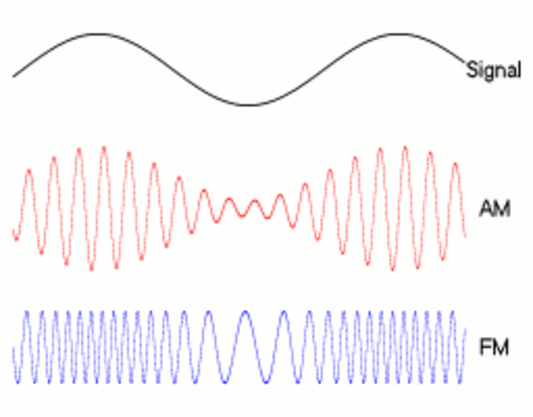
\includegraphics[scale=0.4]{Frequenzaufbereitung/Bilder/Amfm3-en-de.pdf}
% \vspace{-6cm}
%\end{wrapfigure}

\section*{Theorie- und Prüfungsfragen} 

\mucho{1}{TE320}
{Was ist der Baudot-Code?}%Frage
{Es ist ein 7-Bit-Code mit zusätzlichen Start- und Stopbits sowie einem Paritätsbit.}%A
{Es ist ein 8-Bit-Code mit zusätzlichen Start- und Stopbits.}%B
{Es ist ein 5-Bit-Code mit zusätzlichen Start- und Stopbits.}%C
{Es ist ein 5-Bit-Code mit einem Paritätsbit.}%D
{C}%Lösung

\mucho{2}{TE330}
{Wie viel verschiedene Zeichen kann man mit dem 5-Bit Baudot Code erzeugen?}%Frage
{5}%A
{32}%B
{64}%C
{128}%D
{B}%Lösung

\mucho{3}{TE305}
{Wie erfolgt die synchrone Datenübertragung?}%Frage
{Sender und Empfänger synchronisieren ihre Taktfrequenzen mit einem Normalfrequenzsender.}%A
{Sende- und Empfangsstelle werden mit Hilfe der Netzfrequenz in Gleichtakt gebracht.}%B
{Sender und Empfänger werden nach jedem einzelnen Zeichen aufeinander synchronisiert. Die Zeichen enthalten Start- und Stoppbit, die zur Synchronisation dienen.}%C
{Eine Übertragung wird durch eine Synchronisationssequenz eingeleitet. Nach erfolgreicher Synchronisation werden die Pakete aus dem Binärstrom gelesen.}%D
{D}%Lösung

\mucho{4}{TE304}
{Wie erfolgt die Datenübertragung bei Packet-Radio?}%Frage
{Die Daten werden paketweise gesendet. Der Beginn eines Paketes wird durch ein Synchronisationszeichen eingeleitet. Der Takt wird im Empfänger aus den Daten zurückgewonnen.}%A
{Die Daten werden paketweise gesendet. Am Anfang erfolgt ein Startzeichen und am Ende ein Stoppzeichen.}%B
{Die Daten werden parallel ausgesendet. Der Takt wird im Empfänger aus den Daten zurückgewonnen.}%C
{Die Daten werden seriell ausgesendet. Es ist ein asynchrones Verfahren.}%D
{A}%Lösung



\begin{enumerate}
		\item[5] Ordne den 3-dB-Bandbreiten 500Hz, 2.3kHz, 6kHz und 12kHz  eines Quarzfilters die geeignete Verwendung zu (AM, FM, SSB oder CW).\\ \loesung{CW = 500Hz; SSB = 2.3kHz; AM = 6kHz; FM = 12kHz}
	\end{enumerate}

\mucho{6}{TE102}
{Wodurch werden Tastklicks bei einem CW-Sender hervorgerufen? Tastklicks werden hervorgerufen durch}%Frage
{prellende Kontakte der verwendeten Taste}%A
{zu steile Flanken der Tastimpulse}%B
{direkte Tastung der Oszillatorstufe}%C
{ein unterdimensioniertes Netzteil, dessen Spannung beim Auftasten kurzzeitig zusammenbricht}%D
{B}%Lösung

\mucho{7}{TE306}
{Welche HF-Bandbreite beansprucht ein 1200-Baud-Packet-Radio-AFSK-Signal?}%Frage
{25 kHz}%A
{12 kHz}%B
{ca. 6,6 kHz}%C
{ca. 3 kHz}%D
{B}%Lösung

\mucho{8}{TE313}
{Welche HF-Bandbreite beansprucht ein 9600-Baud-FM-Packet-Radio-Signal?}%Frage
{12,5 kHz}%A
{20 kHz}%B
{ca. 6,6 kHz}%C
{ca. 3 kHz}%D
{B}%Lösung

\mucho{9}{TE308}
{Beim Aussenden von Daten in der Betriebsart Packet-Radio muss nach dem Hochtasten des Senders eine gewisse Zeitspanne gewartet werden, bevor mit der Datenübertragung begonnen werden kann. Wie heißt der Parameter mit dem diese Zeitspanne eingestellt wird?}%Frage
{RX-Delay}%A
{DWAIT}%B
{TX-Delay}%C
{Frack}%D
{C}%Lösung

\mucho{10}{TE315}
{Was versteht man bei Packet Radio unter einem TNC (Terminal Network Controller)? Ein TNC}%Frage
{wandelt nur die Töne in digitale Daten und schickt diese an den PC.}%A
{besteht aus einem Modem und dem Controller für die digitale Aufbereitung der Daten.}%B
{wandelt nur die Töne in digitale Daten und schickt diese an den Sender.}%C
{ist ein Modem (Modulator und Demodulator) für digitale Signale.}%D
{B}%Lösung


\mucho{11}{BJ111}
{Was bedeutet die Abkürzung APRS?}%Frage
{Automatisches Positionsmeldesystem}%A
{Automatisches Packet Radio System.}%B
{Amerikanisches Packet Radio System}%C
{Amateurfunk Packet Radio System}%D
{A}%Lösung

\mucho{12}{TE323}
{Welches der folgenden digitalen Übertragungsverfahren hat die geringste Bandbreite?}%Frage
{PSK31}%A
{RTTY}%B
{Pactor}%C
{Amtor}%D
{A}%Lösung